\documentclass[10pt, compress]{beamer}

\usetheme{m}

\usepackage{booktabs}
\usepackage[scale=2]{ccicons}
\usepackage{minted}
\usepackage{tikz}
\usepackage[ruled,vlined,english]{algorithm2e}
\usetikzlibrary{arrows,automata,shapes,positioning,calc}

\usepackage{float} % placement des figures
\usepackage{amssymb} % symboles mathématiques
\usepackage{textcomp} % flèche,  intervalle
\usepackage{stmaryrd} % intervalle entiers
\usepackage{graphicx} % affichage d'images
\usepackage{url} % inclure des urls
\usepackage{forest}

\newcommand{\first}{\texttt{First}}
\newcommand{\last}{\texttt{Last}}
\newcommand{\sort}{\texttt{Sort}}
\newcommand{\triple}{\texttt{Triple}}
\newcommand{\produ}{\texttt{Normalize}}

\newenvironment{exemple}
{\begin{exampleblock}{Example}}
{\end{exampleblock}}

\newenvironment{defi}
{\begin{block}{Definition}}
{\end{block}}

\usepgfplotslibrary{dateplot}

\usemintedstyle{trac}

\title{Platypus, l'outil libre qui répond à vos questions}
\subtitle{}
\date{JDLL 2015}    

\begin{document}

\maketitle

\begin{frame}
    \frametitle{On cherche des réponses}
    \alert{Who was the wife of Louis Pasteur?}
    \begin{figure}
        \includegraphics[width=\textwidth]{pasteurWiki.png}
    \end{figure}
\end{frame}

\begin{frame}
    \frametitle{Outils existants}
    \begin{tabular}{ll}
        WolframAlpha & Marie Pasteur\\
        Google & Article Wikipedia sur Marie Pasteur\\
        Bing & Article Wikipedia Louis Pasteur\\
        Yahoo & Page d'answers.com contenant la question
    \end{tabular}
\medbreak
\alert{Logiciels propriétaire, parfois mauvais...}
\end{frame}

\begin{frame}
    \frametitle{Platypus}
    \begin{center}
        \url{http://askplatyp.us}
        
        \bigskip
        
        \includegraphics[width=0.6\linewidth]{figures/platypus.pdf}
    \end{center}
\end{frame}

\begin{frame}
    \frametitle{Platypus ?}
    \begin{itemize}
        \item<1-> \alert{Open-source}
        \item<2-> \alert{Modulaire}
        \item<3-> \alert{Anglais} pour l'instant
        \item<4-> \alert{Connaissance générale} et math
    \end{itemize}
\end{frame}

\begin{frame}
    \begin{center}
        \Huge Et la démo !
    \end{center}
\end{frame}

\begin{frame}[plain]
    \includegraphics[width=\linewidth]{figures/demo-whoIsAlanTuring.png}
\end{frame}

\begin{frame}[plain]
    \includegraphics[width=\linewidth]{figures/demo-whenIsAlanTuringBorn.png}
\end{frame}

\begin{frame}[plain]
    \includegraphics[width=\linewidth]{figures/demo-whereIsEnsLyon.png}
\end{frame}


\section{Overview}
\begin{frame}[fragile]
    \frametitle{Architecture}
    \begin{figure}
        \includegraphics[scale=.21]{figures/architecture}
    \end{figure}
\end{frame}

\begin{frame}
  \frametitle{Une question}
    \alert{Where does the prime minister of the United Kingdom live?}
\end{frame}

\begin{frame}
 \frametitle{De la question à la forme normale}

\begin{center}
  \alert{Where does the prime minister of the United Kingdom live?}
\end{center}

\begin{figure}
 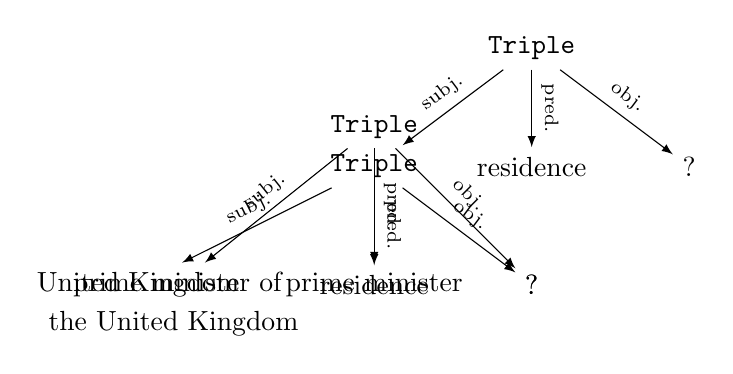
\begin{tikzpicture}
  \onslide<1>{
  \node (7) at (8,9) {$\triple$};
  \node (8) at (5.5,7) {prime minister of};
  \node (11) at (5.45,6.5) {the United Kingdom};
  \node (9) at (8,7) {residence};
  \node (10) at (10,7) {?};

  \draw[->, >=latex] (7) edge node[sloped, anchor=center, above] {\scriptsize{subj.}} (8);
  \draw[->, >=latex] (7) edge node[sloped, anchor=center, above] {\scriptsize{pred.}} (9);
  \draw[->, >=latex] (7) edge node[sloped, anchor=center, above] {\scriptsize{obj.}} (10);}
  
  \onslide<2>{  
  \node (0) at (10,10) {$\triple$};
  \node (1) at (10,8.5) {residence};
  \node (2) at (12,8.5) {?};
  \node (3) at (8,8.5) {$\triple$};
  \node (4) at (8,7) {prime minister};
  \node (5) at (5,7) {United Kingdom};
  \node (6) at (10,7) {?};

  \draw[->, >=latex] (0) edge node[sloped, anchor=center, above] {\scriptsize{obj.}} (2);
  \draw[->, >=latex] (0) edge node[sloped, anchor=center, above] {\scriptsize{pred.}} (1);
  \draw[->, >=latex] (0) edge node[sloped, anchor=center, above] {\scriptsize{subj.}} (3);
  \draw[->, >=latex] (3) edge node[sloped, anchor=center, above] {\scriptsize{subj.}} (5);
  \draw[->, >=latex] (3) edge node[sloped, anchor=center, above] {\scriptsize{obj.}} (6);
  \draw[->, >=latex] (3) edge node[sloped, anchor=center, above] {\scriptsize{pred.}} (4);}
 \end{tikzpicture}
\end{figure}

\end{frame}

\begin{frame}
   \frametitle{Extraction de la réponse : Wikidata}

    Wikidata ?
    \begin{itemize}
        \item \alert{\url{http://www.wikidata.org}}
        \item Une base de \alert{connaissance libre}
        \item \alert{Multilingue}
    \end{itemize}
\end{frame}

\begin{frame}
  \frametitle{Extraction de la réponse : Wikidata}

\begin{figure}
 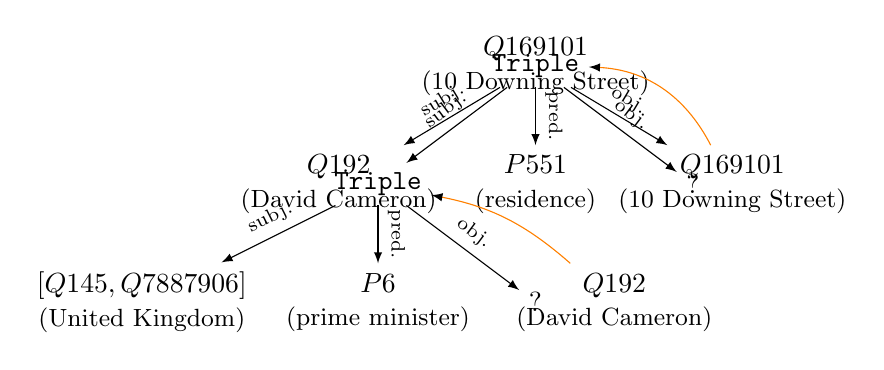
\begin{tikzpicture}
  \onslide<1-4>{\node (0) at (10,10) {$\triple$};}
  \onslide<1-4>{\node (1) at (10,8.5) [align=center] {$P551$\\{\small (residence)}};}
  \onslide<1-3>{\node (2) at (12,8.5) {?};}
  \onslide<1-2>{\node (3) at (8,8.5) {$\triple$};}
  \onslide<1-2>{\node (4) at (8,7) [align=center] {$P6$\\{\small (prime minister)}};}
  \onslide<1-2>{\node (5) at (5,7) [align=center] {$\left[Q145, Q7887906\right]$\\{\small (United Kingdom)}};}
  \onslide<1>{\node (6) at (10,7) {?};}

  \onslide<1-4>{\draw[->, >=latex] (0) edge node[sloped, anchor=center, above] {\scriptsize{pred.}} (1);}
  \onslide<1-3>{\draw[->, >=latex] (0) edge node[sloped, anchor=center, above] {\scriptsize{obj.}} (2);}
  \onslide<1-2>{\draw[->, >=latex] (0) edge node[sloped, anchor=center, above] {\scriptsize{subj.}} (3);}
  \onslide<1-2>{\draw[->, >=latex] (3) edge node[sloped, anchor=center, above] {\scriptsize{subj.}} (5);}
  \onslide<1-2>{\draw[->, >=latex] (3) edge node[sloped, anchor=center, above] {\scriptsize{obj.}} (6);}
  \onslide<1-2>{\draw[->, >=latex] (3) edge node[sloped, anchor=center, above] {\scriptsize{pred.}} (4);}
  
  \onslide<2>{\node (7) at (11,7) [align=center] {\alert{$Q192$}\\\alert{\small (David Cameron)}};}
  \onslide<3-4>{\node (8) at (7.5,8.5) [align=center] {\alert{$Q192$}\\\alert{\small (David Cameron)}};}
  \onslide<4>{\node (9) at (12.5,8.5) [align=center] {\alert{$Q169101$}\\\alert{\small (10 Downing Street)}};}
  \onslide<5>{\node (10) at (10,10) [align=center] {\alert{$Q169101$}\\\alert{\small (10 Downing Street)}};}

  \onslide<3-4>{\draw[->, >=latex] (0) edge node[sloped, anchor=center, above] {\scriptsize{subj.}} (8);}
  \onslide<4>{\draw[->, >=latex] (0) edge node[sloped, anchor=center, above] {\scriptsize{obj.}} (9);}

  \onslide<2>{\draw[->, >=latex] [draw=orange] [bend right=15, above] (7) edge (3);}
  \onslide<4>{\draw[->, >=latex] [draw=orange] [bend right, above] (9) edge (0);}
 \end{tikzpicture}
\end{figure}
\end{frame}


\begin{frame}
    \frametitle{Résultat final}
    \includegraphics[width=\linewidth]{figures/residence-prime-minister.png}
\end{frame}

\begin{frame}
    \frametitle{Recherche simple}
    \includegraphics[width=\linewidth]{figures/10-downing-street.png}
\end{frame}

\begin{frame}
    \frametitle{Math}
    TODO
\end{frame}


\section{Let's sum up}
\subsection{Better than Wolfram?}

\begin{frame}
    \frametitle{Nested question}

Who is the wife of the president of the United States?
    \begin{tabular}{ll}
        \alert{WolframAlpha} & Barack Obama\\
        \alert{Platypus} & Michelle Obama\\
    \end{tabular}

    \medbreak

    \onslide<2->{
        What are the birth dates of the daughters of the wife of the president of the United States?
        \begin{tabular}{ll}
            \alert{WolframAlpha} & Barack Obama\\
            \alert{Platypus} & Saturday, July 4, 1998 \& Sunday, June 10, 2001\\
        \end{tabular}
    }
\end{frame}

\begin{frame}[fragile]
    \frametitle{Conjunction}

Who is the actor of Inception and Titanic?
    \begin{tabular}{ll}
        \alert{WolframAlpha} & all the actors of the two movies\\
        \alert{Platypus} & Leonardo DiCaprio\\
    \end{tabular}
\end{frame}

\subsection{Future work}

\begin{frame}
    \frametitle{Better database}

    ``How fast is the TGV?''

    ``How wide is a tennis court?''

    Not answered by \alert{Wikidata}.

    \medbreak

    $\rightarrow$ Improve Wikidata?

    $\rightarrow$ Use another database?
\end{frame}

\begin{frame}
    \frametitle{Better question parsing}

    ``What is the date of birth of Isaac Newton?''

    ``In which band does Bono sing?''

    Not parsed correctly.

    \medbreak

    $\rightarrow$ Train the Stanford CoreNLP library?

    $\rightarrow$ Improve the algorithm of the Grammatical module?

    $\rightarrow$ Better datasets for the ML modules?
\end{frame}

\begin{frame}
    \frametitle{New modules}
\begin{figure}
 \begin{tikzpicture}
  \node (0) at (-3,2) {\textcolor{mLightBrown}{cooking recipes}};
  \node (0) at (1,1) {\textcolor{mDarkBrown}{HAL}};
  \node (0) at (5,2.5) {\textcolor{mMediumBrown}{meteo}};
  \node (0) at (3,2) {\textcolor{mDarkTeal}{chemistry}};
  \node (0) at (0,0) {\textcolor{mMediumBrown}{programming language interpreter}};
  \node (0) at (-4,-1) {\textcolor{mMediumBrown}{cinema}};
  \node (0) at (0,-2) {\textcolor{mDarkTeal}{music}};
  \node (0) at (4,-1) {\textcolor{mDarkTeal}{literature}};
  \node (0) at (-3,-2) {\textcolor{mDarkBrown}{OEIS}};
  \node (0) at (2,-2.5) {\textcolor{mLightBrown}{translation}};
  \node (0) at (-2,-3) {\textcolor{mMediumBrown}{sport statistics and predictions}};
  \end{tikzpicture}
\end{figure}
\end{frame}

\begin{frame}
    \frametitle{Other ideas...}

    \begin{itemize}
        \item Other languages support (French...)
        \item Improve user experience
        \item Advertise \alert{Platypus}
    \end{itemize}
\end{frame}

\subsection{Conclusion}

\begin{frame}
    \frametitle{Some facts} % to update just before the presentation
    \alert{23 repositories}

    \begin{tabular}{lll}
        6 & PHP & Wikidata libraries and module\\
        12 & Python & Other modules, core, and libraries\\
        1 & C++ & ML-Reformulation\\
        1 & Shell & Deployment scripts\\
        1 & \LaTeX & This presentation and the report\\
        1 & Markdown & The specification\\
        1 & HTML/CSS/Javascript & The Web User Interface\\
        1 & HTML/CSS & The project's website\\
    \end{tabular}

    \alert{1982 commits} (without the ``integration'' repository, which has an automatic commit every 12h)

    \alert{26k lines} of code (13k in PHP, 10k in Python)
\end{frame}

\begin{frame}
    \frametitle{The PPP?}

    \begin{itemize}
        \item A powerful question answering framework
        \item Innovative NLP algorithms
        \item A demo, \alert{Platypus}, with general knowledge and math
    \end{itemize}
\end{frame}


\newlength{\logosize}
\setlength{\logosize}{12pt}
\begin{frame}
    \frametitle{The adventure is only starting...}
    \alert{\url{http://projetpp.github.io/}}

    \begin{tabular}{ll}
        \includegraphics[width=\logosize]{Twitter_logo_blue.png} & \href{https://twitter.com/ProjetPP}{https://twitter.com/ProjetPP}\\
        \includegraphics[width=\logosize]{GitHub-Mark-32px.png} &  \href{https://github.com/ProjetPP}{https://github.com/ProjetPP}\\
        \includegraphics[width=\logosize]{ic_email_black_18dp.png} & \href{mailto:ppp@pony.ovh}{ppp@pony.ovh}\\
    \end{tabular}
\end{frame}


\begin{frame}
    \frametitle{Questions?}
    \begin{center}
        \includegraphics[height=0.7\textheight]{figures/Ornithorhynchus.jpg}
    \end{center}
\end{frame}

\begin{frame}
    \tikzset{
        workpackage/.style={
               node distance = 0.5cm,
               },
    }
    \frametitle{WorkPackages}
    \begin{figure}
        \begin{tikzpicture}
            % PPP members
            \node (rc)                  {Raphaël \textsc{Charrondière}};
            \node (qc)  [below of = rc] {Quentin \textsc{Cormier}};
            \node (tc)  [below of = qc] {Tom \textsc{Cornebize}};
            \node (yh)  [below of = tc] {Yassine \textsc{Hamoudi}};
            \node (mc)  [below of = yh] {Marc \textsc{Chevalier}};
            \node (vl)  [below of = mc] {Valentin \textsc{Lorentz}};
            \node (tpt) [below of = vl] {Thomas \textsc{Pellissier} \textsc{Tanon}};

            % PPP WorkPackages
            \node (reformulation)   [workpackage, right of = rc, right=3cm]  {Reformulation};
            \node (standalone)      [workpackage, below of = reformulation]  {Standalone};
            \node (spellchecker)    [workpackage, below of = standalone]     {SpellChecker};
            \node (communication)   [workpackage, below of = spellchecker]   {Communication};
            \node (grammatical)     [workpackage, below of = communication]  {Grammatical};
            \node (bibliography)    [workpackage, below of = grammatical]    {Bibliography};
            \node (cas)             [workpackage, below of = bibliography]   {CAS};
            \node (datamodel)       [workpackage, below of = cas]            {DataModel};
            \node (architecture)    [workpackage, below of = datamodel]      {Architecture};
            \node (core)            [workpackage, below of = architecture]   {Core};
            \node (sysadmin)        [workpackage, below of = core]           {System Administration};
            \node (wikidata)        [workpackage, below of = sysadmin]       {Wikidata};
            \node (webui)           [workpackage, below of = wikidata]       {WebUI};

            % Edges
            \path (reformulation.west)   edge (rc.east)
                  (standalone.west)      edge (qc.east)
                  (spellchecker.west)    edge (tc.east)
                  (communication.west)   edge (tc.east)
                  (grammatical.west)     edge (tc.east)
                  (grammatical.west)     edge (yh.east)
                  (bibliography.west)    edge (yh.east)
                  (datamodel.west)       edge (yh.east)
                  (datamodel.west)       edge (mc.east)
                  (datamodel.west)       edge (vl.east)
                  (datamodel.west)       edge (tpt.east)
                  (architecture.west)    edge (mc.east)
                  (architecture.west)    edge (vl.east)
                  (architecture.west)    edge (tpt.east)
                  (cas.west)             edge (mc.east)
                  (core.west)            edge (vl.east)
                  (sysadmin.west)        edge (vl.east)
                  (wikidata.west)        edge (vl.east)
                  (wikidata.west)        edge (tpt.east)
                  (webui.west)           edge (tpt.east);
        \end{tikzpicture}
    \end{figure}
\end{frame}


\end{document}
